%aum gaanathipathaye namaha
%srj
\section{Methodology}\label{sec:methodology}
This section, we present the four modules in \tool in details.
As the first step, \tool disassembles the binary and splits it into basic functional units or functions. Then, it constructs the control-flow graph (CFG) from each function, where each CFG is consists of one or more basic-blocks. Later, constructed CFGs are used to generate partial execution traces. The definitions of CFG and basic-block are given below:

\begin{mydef}
\emph{(\textbf{Basic-block}) }  A sequence of assembly instructions without any jumps or jump targets in the middle, where a jump target starts a block, and a jump ends a block.
\end{mydef}
\begin{mydef}
\emph{(\textbf{Control-flow graph}) } A directed graph, where each node represents a basic-block and edges represent control flow.
\end{mydef}

\subsection{Partial Trace Extraction - \todo{completed}} \label{subsec:partial_trace}

In the literature ~\cite{pewnycross,lakhotia2013fast,ruttenberg2014identifying}, basic-block is considered as a single building block. However, it is too restrictive to assume that a function compiled for two different compiler optimization-level (or compiled using two different compilers or in the worst, compiled for two different architectures) will maintain the same basic-block structure. That is basic-block based function modelling lacks the granularity, which is vital for cross-architecture and -platform function search. Hence, to overcome this limitation, in \tool, we propose a partial trace based function modelling, which is more flexible in terms of granularity. That is, from each function, we generate partial traces of various lengths, where by varying the length, the granularity of single building block is adjusted\footnote{length of one yields a basic-block based models, where the basic-block is considered as a single building block}


Partial trace is a sequence of adjacent basic-blocks that lie along a program execution path. Partial traces can be of any length, for example, partial trace of length 2 is a concatenation of two adjacent basic-blocks along the program CFG. Our partial trace extraction is based on the technique proposed in \cite{david2014tracelet}, where partial trace of size \textit{k} referred to as \textit{k-tracelet}. Formal definition of \textit{k}-tracelet \cite{david2014tracelet} is given below.

\begin{mydef}
\emph{\textbf{(\textit{k}-tracelet)}} k-tracelet is an ordered tuple of k sequences, each representing one of the basic-blocks in a directed acyclic sub-path in the CFG, and containing all of the basic-blocks assembly instructions \cite{david2014tracelet}.
\end{mydef}

To be self-contained, we briefly explain the partial trace (or \textit{k}-tracelet) extraction algorithm presented in \cite{david2014tracelet}. Algorithm~\ref{algo:k-trace} shows the steps involved in extracting \textit{k}-tracelets from a CFG. The tracelets are extracted recursively from the nodes in the CFG. To extract all the \textit{k}-traclets from a certain node in the CFG, we compute all (\textit{k-1})-tracelets from any of its \textit{sons}, and use a Cartesian product (\texttt{X}) between the node and the collected tracelets. Algorithm 2 uses a helper function, \texttt{StripJumps}. This function takes a sequence of assembly instructions in which a jump may appear as the last instruction, and returns the sequence without the jump instruction. 
\note{That is, in partial traces, the flow of execution is already determined and hence, all control-flow instructions (e.g., \texttt{jmp}, \texttt{je}, \texttt{jnz}, \ldots) are omitted}. 
For example, figure \ref{fig:example-cfg} depicts a sample CFG of a function and figure \ref{fig:ex-tracelet} presents the extracted partial traces (for $\textit{k} = 3$). From the partial traces it can be see that the original control-flow instructions (\texttt{jnx xxx}, \texttt{jb xxx} and \texttt{jb xxx}) are omitted as the flow of execution is already determined. It is important to note that the feasibility of the flow of execution is not considered when generating the partial traces. However, later in the section, we'll explain how we remove the partial traces that are totally \textit{infeasible} (i.e., the flow of execution is infeasible) with the help of a constraint solver.  




\begin{MyAlgo}[!ht]{-4.9cm} %increase or decrease margin, span across columns
 \DontPrintSemicolon
 \KwData{control-flow graph $CFG$}
 \KwResult{set of k-tracelets $kT$}
 \SetKwFunction{algo}{ExtractTracelets}\SetKwFunction{proc}{Extract}
 \SetKwProg{myalg}{Algorithm}{}{}
 \myalg{\algo{$CFG$}}{
  $kT \longleftarrow \emptyset$ \tcp*{set of partial traces}
 \ForEach{{\upshape basic-block} b {\upshape in} $CFG$}{
  %\tcc{write the algo here}
  $kT \longleftarrow kT \cup Extract(b, k)$\;
  }
  \Return ${ kT}$
  }
  \setcounter{AlgoLine}{0}
  \SetKwProg{myproc}{Procedure}{}{}
  \myproc{\proc{b, k}}{
  $b_s \longleftarrow StripJumps(b)$\;
  \eIf{$k == 1$}{
    \Return $b_s$
  }{
   \Return $\bigcup b \times Extract(b^\prime, k-1)$\;
  }
  }
 \caption{Partial trace extraction from a fucntion CFG}\label{algo:k-trace}
\end{MyAlgo}

\begin{figure}[!h]
\begin{center}\vspace{-1mm}
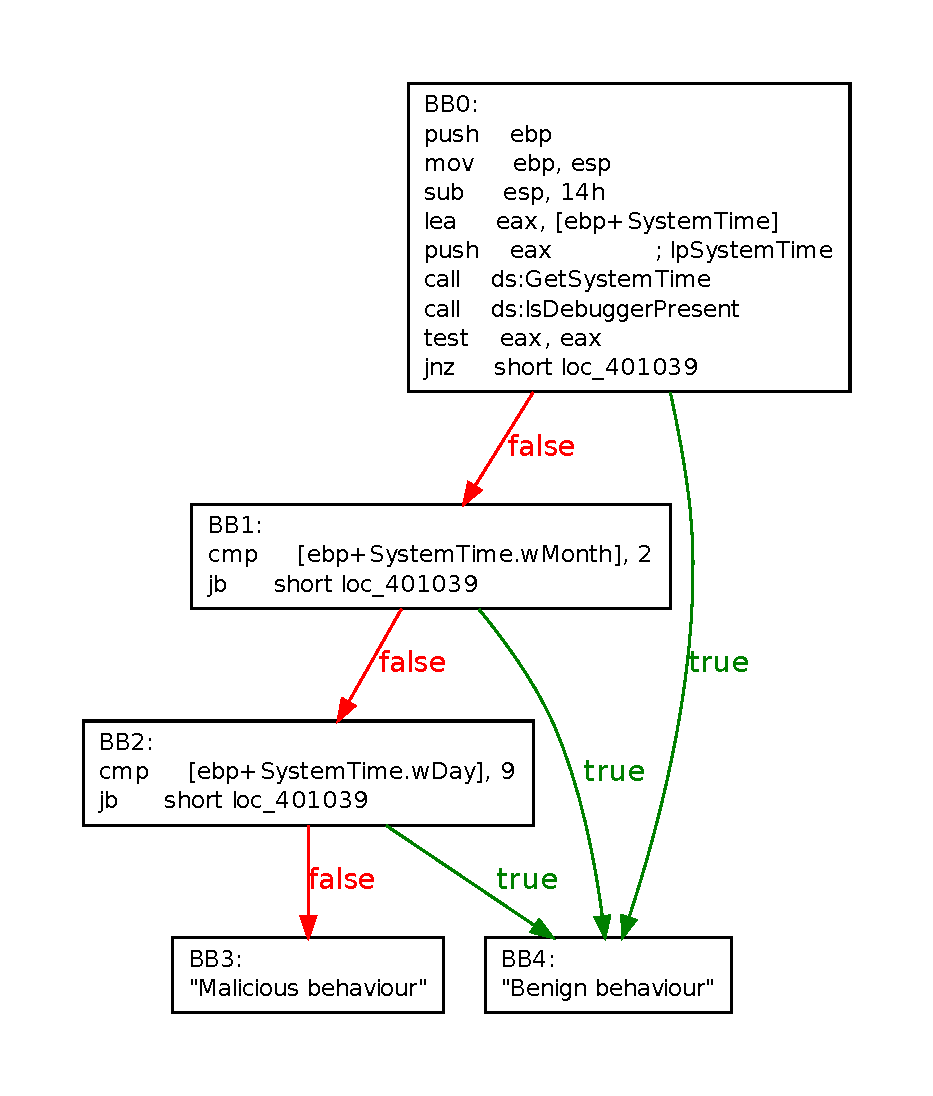
\includegraphics[height=6cm, width=5.5cm]{srj-figures/srj-toy_malware_cfg.pdf} \vspace{-1mm}
\caption{Sample CFG of a function}
\label{fig:example-cfg} \vspace{-1mm}
\end{center}
\end{figure}

\begin{figure}[!h]
\scriptsize
  \begin{subfigure}[b]{0.5\linewidth}
    \centering
   % \includegraphics[width=0.75\linewidth]{srj-figures/srj-hierarchy-2.png}
    \raggedright{\textbf{\texttt{
    \\
    	push ebp\\
    	mov	ebp, esp\\
   		sub	esp, 14h\\
   		lea eax, [ebp+SysT]\\
   		push eax\\
   		call ds:LibCall1\\
   		call ds:LibCall2\\
   		test eax, eax\\
   		%jnz short loc\_401039\\
   		cmp [ebp+SysT.wMonth],2\\
   		%jb short loc\_401039\\
   		cmp [ebp+SysT.wDay],9\\
   		%jb short loc\_401039
    }}}
    \caption{\small{Tracelet $\langle BB0, BB1, BB2\rangle$}}
   \label{fig:traceleta}
    \vspace{4ex}
  \end{subfigure}%%
  \begin{subfigure}[b]{0.5\linewidth}
    \centering
      \raggedright{\textbf{\texttt{
    \\
    	push ebp\\
    	mov	ebp, esp\\
   		sub	esp, 14h\\
   		lea eax, [ebp+SysT]\\
   		push eax\\
   		call ds:LibCall1\\
   		call ds:LibCall2\\
   		test eax, eax\\
   		%jnz short loc\_401039\\
   		cmp [ebp+SysT.wMonth],2\\
   		%jb short loc\_401039\\
   		benign behaviour
    }}}
    \caption{\small{Tracelet $\langle BB0, BB1, BB4\rangle$}}
    \label{fig:traceletb}
    \vspace{4ex}
  \end{subfigure}
  \begin{subfigure}[b]{0.5\linewidth}
    \centering
    \raggedright{\textbf{\texttt{
    \\
   		cmp [ebp+SysT.wMonth],2\\
   		%jb short loc\_401039\\
   		cmp [ebp+SysT.wDay],9\\
   		%jb short loc\_401039\\
   		benign behaviour
    }}}
    \caption{\small{Tracelet $\langle BB1, BB2, BB4\rangle$}}
    \label{fig:traceletc}
  \end{subfigure}%%
  \begin{subfigure}[b]{0.5\linewidth}
    \centering
   \raggedright{\textbf{\texttt{
    \\
   		cmp [ebp+SysT.wMonth],2\\
   		%jb short loc\_401039\\
   		cmp [ebp+SysT.wDay],9\\
   		%jb short loc\_401039\\
   		malicious behaviour
    }}}
    \caption{\small{Tracelet $\langle BB1, BB2, BB3\rangle$}}
    \label{fig:traceletd}
  \end{subfigure}
  \\
  \caption{Tracelets extracted from the CFG shown in figure \ref{fig:example-cfg}\\.\\}
  \label{fig:ex-tracelet}
\end{figure}


\subsection{Semantic Model Generation} \label{subsec:sem_mod}
%These code properties act as contextual information for the vulnerability.

%\todo {\color{blue} Define code property and explain each of the following in details with some examples.}
Due to the dramatic difference in the syntax representations of the binary generated from different compilers, architectures and platforms,
\tool leverage on two types of semantic models, generated from partial traces, to extract semantic features: (1) state-based semantic model and (2) abstract semantic model. As discussed later, each model complement each other on extracting semantic features, which are later fed into the machine learning framework. State-based semantic model gives the low-level perspective of the function (e.g., the effect of a function on the memory, flags and registers), whereas abstract-semantic model gives the high-level intentions of the function (e.g., the high-level operations carried out by the function). In the following sub sections, we'll elaborate on them in detail.
%These complementing features summarize the behavior of the same binary code at different levels to achieve an accurate and yet robust matching cross compilers, architectures and platforms.
%under investigation so that they complement each other and give better understanding of the program.
%On the other hand, syntactic features try to explain the high-level behavioural aspects of the binary code (e.g., type of operation carried out, such as data movement or arithmetic operation).


\subsubsection{State-based Semantic Modelling - \todo{completed}} \label{subsubsec:stat_sem}
State-based semantic model aims to capture the execution effect of the binary code in terms of machine state updates. Lets consider the following simple machine (adapted from \cite{de2015micro}) using which we explain the state-based semantic modelling.

%\subsubsection*{Simple Machine} \label{subsubsubsec:bas_mach}
Assume this simple machine has a fixed word size and a fixed set of general-purpose registers, conditional flag registers and a program counter (\textit{pc}) register. Consider the following (subset of) common instructions of the machine:
\begin{equation*}
inst ::= \mathsf{Mov} \: r_s\, r_d\; \vert \; \mathsf{Binop_\otimes} \: r_1\, r_2\, r_d\,f_d \; \vert \; \mathsf{Load} \: r_p\, r_d\; \vert \; \mathsf{Store} \: r_p\, r_s 
\end{equation*}
where $\otimes \in \lbrace \div, \times, \leq, \geq, \ldots\rbrace$. A machine state is characterised by a tuple\footnote{It is noted that in the original formalization, in \cite{de2015micro}, \textit{flag} is not included. However, as our models are generated from partial traces, its is essential to consider the state of conditional flags (e.g., $CF, PF, \ldots$) in similarity computation} ($mem, reg, flag, pc$) of a word-addressable memory \textit{mem} (a partial function from words to words), a register file \textit{reg} (a function from register names to words), a conditional flag file \textit{flag} (a function from flags names to words) and a pc value (a word). Note that the memory is a partial function; trying to address outside of the valid memory (by trying to fetch the next instruction from an invalid address, or loading from or storing to one) halts the machine.

A typical step rule for this machine is written like this:
\begin{equation*}
\begin{aligned}
\mathnormal{\frac{ \splitfrac{mem[pc]=i \quad decode \: i = \; \mathsf{Binop_\otimes} \: r_1\, r_2\, r_d\,f_d \quad reg[r_1]=w_1}{\splitfrac{reg[r_2]=w_2 \quad reg^\prime = reg[r_d \leftarrow w_1 \otimes w_2]}{flag^\prime = flag[f_d \leftarrow w_1 \otimes w_2]\hfill}\hfill \mathsf{(Binop)}}}{(mem, reg, flag, pc) \rightarrow (mem, reg^\prime, flag^\prime, pc+1)}}
\end{aligned}
\end{equation*}

Let's read this rule in detail. Looking up the memory word at address \textit{pc} yields the word \textit{i}, which should correspond to some instruction (i.e., an element of the \textit{inst} set defined above)via  partial function \textit{decode}.  In this case, that instruction is $\mathsf{Binop_\otimes} \: r_1\, r_2\, r_d\, f_d$. Registers $r_1$ and $r_2$ contain the operands $w_1$ and $w_2$, respectively. The notation $reg[r_d \leftarrow w_1 \otimes w_2]$ denotes a partial function that maps $r_d$ to $w_1 \otimes w_2$ and behaves like $reg$ on all other arguments. Similarly, $flag[f_d \leftarrow w_1 \otimes w_2]$ denotes the partial function that maps $f_d$ to the side-effects (if any) of $w_1 \otimes w_2$ on the conditional flags. The next machine state is calculated by updating the register and conditional flag files, incrementing the pc, and leaving the memory unchanged. 

The step rule for $\mathsf{Store}$ instruction can be written as follows: 
\begin{equation*}
\begin{aligned}
\mathnormal{\frac{ \splitfrac{mem[pc]=i \quad decode \: i = \; \mathsf{Store} \: r_p\, r_s \quad reg[r_p]=w_p}{reg[r_s]=w_s \quad mem^\prime = mem[w_p \leftarrow w_s] \hfill}\mathsf{(Store)}}{(mem, reg, flag, pc) \rightarrow (mem^\prime, reg, flag, pc+1)}}
\end{aligned}
\end{equation*}
where it stores the value contained in the register $r_s$ in the memory location pointed to by the register $r_p$. The next state is calculated by updating the memory, incrementing the pc and leaving the register and conditional flag files unchanged. Similarly, we can write the step rule for all other instructions supported by the machine. 
\todo{include the step rule for all instructions - overkill?}
%\todo{Write a step rule that modifies the }
~\\
\\
The updates made by an instruction on the machine state (as shown by step rules above) are represented by a quantifier-free bit-vector (QFBV) formula.  That is, the function $\langle\!\langle \cdot \rangle\!\rangle$ converts an instruction-sequence into a QFBV formula. The methodology for this conversion can be found elsewhere \cite{lim2011symbolic}. QFBV formula for an instruction sequence is a  2-vocabulary formula that specifies a state transformation 
%(i.e., $\langle$pre-state$\rangle \rightarrow \langle$post-state$\rangle$)
, where the primed vocabulary (e.g., $\textit{mem}^\prime$) is the post-state vocabulary, and the unprimed vocabulary (e.g., \textit{mem}) is the pre-state vocabulary. It is important to note that in QFBV formulas the state transition of the program counter \textit{pc} (i.e., $pc^\prime = pc+1$) is omitted as it doesn't not contribute to compare two different programs. Hence, in \tool, the machine state is essentially characterised by a triple (\textit{mem, reg, flag}).
\note{We generate QFBV formulas for the entire partial trace, hence, state of \textit{pc} plays an insignificant role in semantic matching.}

The QFBV formulas for a few IA-32 instructions are given in figure \ref{fig:example-qfbv}. The first instruction loads the value in the memory location pointed to by the base-pointer (i.e.,  $\mathtt{EBP}$) to the  $\mathtt{EAX}$ register. The second instruction pushes the 32-bit constant value 0 on the stack and the third instruction loads  $\mathtt{EAX}$ with the value  $\mathtt{EBP+4}$ (without modifying the value of any flag).


\begin{figure}[!h]
\begin{center}\vspace{-1mm}
%\scriptsize
\begin{itemize}
  \item[] $\mathtt{\langle\!\langle mov \;\; eax, [ebp]\rangle\!\rangle\equiv EAX^\prime = Mem(EBP)}$
  \item[] $\mathtt{\langle\!\langle push \;\; 0\rangle\!\rangle\equiv ESP^\prime=ESP-4 \wedge Mem^\prime = Mem[ESP-4\mapsto 0]}$
  \item[] $\mathtt{\langle\!\langle lea \;\; eax, [ebp+4]\rangle\!\rangle\equiv EAX^\prime = EBP + 4}$
\end{itemize}
~\\
\caption{QFBV formulas for example IA-32 instructions}
\label{fig:example-qfbv}
\end{center}
\end{figure}
Functions, in a real-world program, can easily have several thousand instructions and hence, it is not practical, in terms of scalability, to compare each instruction in the signature function with the target function. In addition, comparison of single instructions will result in high false positive rate, where an instruction can be too common and too small to capture the underlying function semantics.  For example, the instruction \texttt{mov eax, [ebp]}, in its own, does not tell anything about the function and can appear in functions that are totally dissimilar.  Therefore, in \tool, we capture the effect of each partial trace (not single instructions) has on the machine state 
%register, flag and memory locations written to or updated 
during execution.
\note{It is important to note that partial traces, in general, have lots of inputs (i.e., registers, flags and memory locations read from, called \textit{input arguments}) and outputs (i.e., registers, flags and memory locations written to, called \textit{output arguments}). Hence, from extracted QFBV formulas, the input and output arguments are identified and they are 
%organized in such a way that output arguments are expressed by input arguments}.
represented in the form: $\langle$output argument$\rangle$ $=\langle$input argument(s)$\rangle$. The relationship between input and output arguments are called \textit{symbolic expressions}.}.
%That is, using QFBV formulas, we capture the machine-state transitions over each partial trace, resulting in a \texttt{set} of $\langle$pre-state, post-state$\rangle$ pairs for each function under investigation.  

%That is, we accumulate the QFBV formulas over a partial trace and derive an expression (called, symbolic expression or S-Expression) for each register, flag and memory locations written to during the execution.  

%the QFBV formulas are accumulated over a rage of basic-blocks (in our case, partial traces) and from the accumulated QFBV formulas, the effect of

%That is, from each partial trace, QFBV formulas are collected and using them the effect of   
 
%A program state is characterised by register, control flag and memory values.
%Formally, we define a program state as a triple $$(RegMap, FlagMap, MemMap)$$
%where $RegMap$, $FlagMap$, and $MemMap$ map each register, control flag, and memory location to a value, respectively.
%The effect of a binary code on the program states, is represented by a set of symbolic formulae, called \textit{symbolic expressions}.
%
%%\begin{mydef}
%%\emph{(\textbf{Symbolic Expression}) } Symbolic formulae that represent the effects of executing a piece of code, on the program-state, in-terms of system registers, control flags and memory values.
%%\end{mydef}
%\begin{eqnarray}
%\label{eq:sym_exp}
% \text{\texttt{push ebp}} &\equiv& \text{(\texttt{(ESP' = ESP-4})} ~\wedge \nonumber \\
%   &&  \text{(\texttt{[ESP-4] = EBP})}~
%\end{eqnarray}
%For example, the symbolic sexpression of an instruction `\texttt{push ebp}' is shown in Equation \ref{eq:sym_exp} (assuming in an IA-32 machine). It can be seen that when \texttt{EBP} register is pushed into the stack, the value of \texttt{ESP} register changes to \texttt{ESP-4} and the memory location \texttt{[ESP-4]} is now holding the value of \texttt{EBP} register. Here, prime (\texttt{'}) indicates the post execution state. In contrast to other symbolic expression\footnote{Symbolic expression and semantic features are used interchangeably in this paper.} based program representation techniques~\cite{pewnycross,lakhotia2013fast,ruttenberg2014identifying}, we extract semantic features at various granularity levels (i.e., beyond basic-block levels) to measure the effect of partial traces at different program points. Partial trace models are explained in details later under function model generation module.

%\note{discuss the memory reads and writes briefly}

\subsubsection{Abstract Semantic Modelling \todo{Unified Semantic Abstraction?}} \label{subsubsec:abs_sem_mod}

The limitation in state-based semantic model is that it lacks some of the details, readily available from the machine code, that can be leveraged on to understand the intentions (or objectives) of the partial traces. That is, state-based models are too low-level as such they are incapable of capturing the high-level intentions of the partial traces. In addition, the effects of library calls are not interpreted in state-based models. That is, the instructions \texttt{call CreateFile} and \texttt{call GetTime} are treated in the same way, whereas, in reality, the effects of these two library calls are totally different. Hence, in \tool, we compensate the limitations of state-based semantic models using abstract semantic models, where we capture the high-level intentions, of each partial trace, using \textit{abstract semantic} graphs. Next, we explain the high-level intentions (or objectives) in details.


\subsubsection*{High-level Intentions} 
The instructions extracted from  machine code can be directly used to represent the high-level intentions. For example, \texttt{mov eax ebx} tells us that the value in source register \texttt{ebx} copied to the destination register \texttt{eax}. Similarly, the instruction \texttt{call CreateFile} indicates that a new file is created (or an existing file is opened). However, this representation shamelessly fail in the event of cross-architecture and -platform experiments due to the differences in instruction set architectures and the difference in library calls, supported by different platforms. Therefore, to overcome these limitation, in abstract semantic models, the high-level intentions are characterised by two behavioural abstractions: (1) \textit{operation type}, and (2) \textit{library call type}. That is, instead of using instructions and library calls directly to represent the high-level intentions, we leverage on their abstractions.

\begin{table}[t]
\caption{Categorization of assembly instructions based on their high-level operations. \textsuperscript{$\spadesuit$}A common trick to move 0 to a register is by \texttt{xor}ing the register with itself, similarly, \texttt{lea} can be used to perform arithmatic operations}\label{tab:opt-cat}
\begin{center}
{\scriptsize
\begin{tabular}{|c|c|}
  \hline
  \textbf{Operation type} & \textbf{Sample instructions} \\
  \hline
  Data movement & \texttt{mov, movsx, xchg, xor\textsuperscript{$\spadesuit$}}\\
  \hline
  Arithmetic  & \texttt{add,adc,sub,sbb, lea\textsuperscript{$\spadesuit$}} \\
  \hline
  Logic & \texttt{and,or,not,xor}\\
  \hline
  Shift-rotate & \texttt{shr,shl,sal,rcl,rcr}\\
  \hline
  String  & \texttt{cmps,cmpsb,cmpsw,cmpsd} \\
  \hline
  %Loop & \texttt{loop,loopne,loopnz,loope}\\
  %\hline
  %Control transfer & \texttt{jno,jnp,jns,jo,jp,jpe}\\
  %\hline
  Stack  & \texttt{pusha, pushf, popa, popf} \\
  \hline
  Conversion & \texttt{cbw, cwd, cwde, cdq, csq}\\
  \hline
  %I/O  & \texttt{in, out} \\
  %\hline
 %Floating-point & \texttt{fld, fstp}\\
  %\hline
 % Halt & \texttt{hlt}\\
 % \hline
 Flag  & \texttt{cld,clc,stc,std,sti} \\
  \hline
  \end{tabular}
}
\end{center}
\end{table}

\begin{table}[t]
\caption{Categorization of library calls based on their high-level operations}\label{tab:lib-cat}
\begin{center}
{\scriptsize
\begin{tabular}{|c|c|}
  \hline
  \textbf{Library call type} & \textbf{Sample library calls} \\
  \hline
  String & \texttt{strcpy, strcat}\\
  \hline
  Memory  & \texttt{memcpy, memset} \\
  \hline
  Network & \texttt{socket, gethostbyname }\\
  \hline
   File & \texttt{CreateFile, fopen}\\
  \hline
  Process  & \texttt{CreateProcess, pthread\_exit} \\
  \hline
 Crypto & \texttt{crypt, encrypt}\\
  \hline
  Synchronization  & \texttt{CreateMutex, pthread\_mutex\_init} \\
  \hline
  Heap & \texttt{brk, HeapAlloc}\\
  \hline
  \end{tabular}
}
\end{center}
\end{table}

%In addition to low level semantic features, \tool leverages on high-level semantic features extracted from the functions to understand the operations carried out by the binary code. Combining state-based semantic and abstract semantic features gives the good mix of functions properties that can be effectively used to search similar functions from the target function pool. To this end, we are considering two behavioural abstractions: (1) operation type, and (2) library call invocations.

\begin{itemize}

\item \textbf{Operation type}: Here, we look into the actual machine code to infer the possible operations, at a given abstraction level, that a partial trace can perform. To this end, we have identified several types of operations that are architecture agnostic. That is, these operation types are uniform across different architectures. They are as follows: data movement, arithmetic operation, logic operation, shift and rotate operation, string operation, 
%loop operation, control transfer operation, 
stack operation, conversion (or sign extension) operation, 
%I/O operation, 
floating-point operation 
%halt operation 
and flag manipulation. Table \ref{tab:opt-cat} list the operation types used in \tool.

\item \textbf{Library call type}: Library call invocations give a valuable hint about the activities that are likely to be carried by the partial trace. For example, the presence of \texttt{strcpy} function from \texttt{libc} library indicates that the partial trace is likely to handle strings. We can directly include the library call as part of the feature, if both the search query and the target functions are compiled for the same platform (e.g., Linux) and uses the identical library calls. However, in real-world, this assumption is too restrictive, even within the same platform, as there are several alternate library calls available to accomplish a given task  (e.g., in Windows, to create a file, a programmer can either use \texttt{CreateFile} library call or \texttt{OpenFile} with open switch).  Thus, in abstract semantic models, to account for the differences in function calls that accomplish similar task and to enable cross-platform (e.g., Windows vs. Linux) analysis, we map library calls to their corresponding types. For example, string functions such as \texttt{strlen} and \texttt{srtncat} are mapped to \texttt{string} call type. Table \ref{tab:lib-cat} lists the library call types used in \tool.
\end{itemize}

\subsubsection*{Abstract Semantic Graph} 
The high-level intentions extracted from partial traces alone is not very useful unless it is represented systematically to capture the complete picture. For example, consider the following instruction sequence and the corresponding abstractions.

\begin{itemize}
\itemsep0em 
  \item[] $\mathtt{mov \;\; eax, [ebp] \quad\quad// data\_movement\_from\_memory}$
  \item[] $\mathtt{push \;\; eax \quad\quad// stack\_operation\_store}$
  \item[] $\mathtt{call \;\; socket \quad\quad// network\_connection}$
\end{itemize}
 
It can be seen that abstract information extracted from each instruction alone, without any systematic representation, doesn't fully express the underlying intention of this code segment. One major drawback in just extracting the high-level intentions is that the relationship between intentions are completely ignored, where in the above code segment, all three instructions are related. Hence, its vital to reflect the relationship between extracted intentions. To this end, we use directed graph to represent the high-level intentions and their relationship. It is called an abstract semantic graph and the definition is given below.

\begin{mydef}
\emph{(\textbf{Abstract Semantic Graph}) }  Abstract Semantic Graph is a directed acyclic graph, where the nodes represent the high-level intentions and the edges represent the relationship between two intentions. Here, relationship refers to the data dependence between two intentions.
\end{mydef}

It is important to note that identifying the data-dependence relationship between two intentions is not feasible as the extracted intentions are too abstract, hence, building the abstract semantic graph, we leverage on the data-dependence between assembly instructions and propagate the relationship to the intentions level. This is from the notion that if two assembly instructions are data-dependent, their high-level abstractions (i.e., intentions) are also data-dependent. To this end, we rely on the \textit{def-use} chains to identify the data-dependence. The abstract semantic graph for the above code segment will look like this: 

\begin{figure}[!h]
\begin{center}\vspace{-1mm}
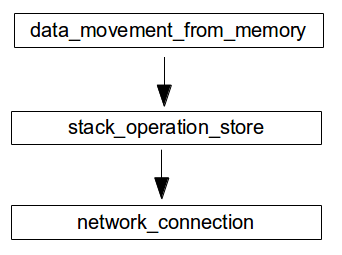
\includegraphics[height=4cm, width=6cm]{srj-figures/srj-graph.png} \vspace{-1mm}
\caption{Abstract semantic graph}
\label{fig:abs} %\vspace{-1mm}
\end{center}
\end{figure}

\begin{MyAlgo}[!ht]{-4.9cm} %increase or decrease margin, span across columns
 \DontPrintSemicolon
 \KwData{partial trace $PT$}
 \KwResult{set of abstract semantic graphs $G$}
% \SetKwFunction{algo}{ExtractTracelets}\SetKwFunction{proc}{Extract}
% \SetKwProg{myalg}{Algorithm}{}{}
% \myalg{\algo{$CFG$}}{
  $G \longleftarrow \emptyset$ \;%\tcp*{set of abstract semantic graphs}
 \ForEach{{\upshape instruction} i {\upshape in} $PT$}{
  %\tcc{write the algo here}
  %$kT \longleftarrow kT \cup Extract(b, k)$\;
  $D_i \longleftarrow  getDef(i)$\;
  $g := {}$\;
  $j := i + 2$\;
   \ForEach{{\upshape instruction} j {\upshape in} $PT$}{
   $U_j \longleftarrow  getUse(j)$\;
   $K_j \longleftarrow  getKill(j)$\;
   \If{$U_j \in D_i $}{
	   	$g := g \cup {v_i \rightarrow v_j}$\; 
   		 \If{$getType(j) == COPY$}{
   			$D_i := D_i \cup getDef(j)$\;
   		}
     }
      \If{$K_j \in D_i $}{
	   	$D_i := D_i \setminus K_j$\;
   		}
   		\If{$D_i ==  \emptyset $}{
   			\If{$g$ {\upshape not in}  $G$}{
   		 		$G := G \cup g$\; 
   		 	}
	   	   break\;
   		}
   }
  }
  \Return ${G}$
  %}
  %\setcounter{AlgoLine}{0}
  %\SetKwProg{myproc}{Procedure}{}{}
  %\myproc{\proc{b, k}}{
  %\eIf{$k == 1$}{
   % \Return $b_s$
  %}{
   %\Return $\bigcup b \times Extract(b^\prime, k-1)$\;
  %}
  %}
  \\
 \caption{Abstract semantic graph constraction using def-use chains}\label{algo:def-use}
\end{MyAlgo}

From figure \ref{fig:abs}, it can be seen that the relationship between high-level intentions gives the complete picture of what the code segment is doing. That is, from the above abstract semantic graph, we can infer that some data from the memory is sent over the network.  
%Thought these code properties helps to identify potential candidate functions in the target program, there are several drawbacks that we need to be aware of. First, it is important to note that some programs may implement their own version of some the library functions, in which case, we may fail to detect the vulnerabilities in functions (if present) that invoke their own version of library function. Fortunately, most of programs still use the standard library functions and thus, we decided to include them as part of the pre-filtering properties. Next, structural information, cannot always be trusted as, in practise, compilers can inline/outline functions and hence, this metric will provide some misleading information. Similarly, operation type may too provide some false indication as some tasks can be achieved with semantically equivalent instruction that belongs two different types in our categorization.

%However, considering the number of functions present in the real world applications, it is very beneficial, in terms of scalability, to have a pre-filtering process in place to select candidate target functions that are likely to contain vulnerability.   Hence, to reduce the negative impact of our properties, we apply weights to each property based on their contribution in pre-filtering. Through evaluation, we identified that library call invocation and operation type properties considerably contributes towards correctly identifying candidate target functions followed by structural property. Therefore, the total synthetic similarity ($sim_{tot}$) is measured as follows:
%\begin{equation}
%sim_{tot} = w_l*sim_l + w_o*sim_o + w_s*sim_s \label{eq:tot_syn_sim}
%\end{equation}
%where, $sim_l$, $sim_o$ and $sim_s$ refers to similarities based library call invocation, operation type and structural properties, and $w_l$, $w_o$ and $w_s$ refers to their corresponding weights, respectively.

\subsection{Semantic Feature extraction \todo{Provide example?}} \label{subsec:sem_fea_ext}
In this section, we explain the feature extraction process from state-based semantic models and abstract semantic models in details.

\subsubsection{Feature extraction from state-based semantic models} \label{subsubsec:sb_sem_mod_fe}
As discussed in section \ref{subsubsec:stat_sem}, partial traces are represented as collection of symbolic expressions. However, the extracted symbolic expressions cannot be directly fed into our machine learning module. Hence, we leverage on the constraint solver to extract features by solving the symbolic expressions. Here, solving refers to finding appropriate concrete values for symbolic inputs (or input arguments) such that all the constraints are satisfied. Later, using these concrete inputs, the corresponding concrete values are obtained for all output arguments.

It is important to note that in sample-based feature extraction technique, proposed in the literature ~\cite{pewnycross}, the relationship between two symbolic expressions are ignored, where each expression is resolved separately independent of each other. On the    other hand, in our approach, we consider the relationship among symbolic expressions. For example consider the following symbolic expressions:
\begin{itemize}
\centering
\itemsep0em 
  \item[] $\mathtt{EAX = EDX + 0x5}$
  \item[] $\mathtt{ECX = EAX + EBX}$
\end{itemize}


From the above symbolic expressions, it can be seen that both are related via the register $\mathtt{EAX}$. That is, output argument of first symbolic expression (i.e., $\mathtt{EAX}$) is passed as one of the input arguments to the second symbolic expression. Therefore, we can infer that $\mathtt{ECX}$ register depends on $\mathtt{EAX}$, $\mathtt{EBX}$ and $\mathtt{EDX}$ registers. However, this relationship is missing in sample-based feature extraction technique, where for a given value of $\mathtt{EDX}$ register, the value of $\mathtt{EAX}$ register is computed and for a given value of $\mathtt{EAX}$\footnote{Not necessarily the value computed for $\mathtt{EAX}$ register in the first expression is used in the second expression} and $\mathtt{EBX}$ registers, the value of $\mathtt{ECX}$ register is computed. In \tool, the order of symbolic expression irrelevant as the constraint solver accumulate all the symbolic expressions generated from a partial trace before it generates a model that satisfy all the constraints.

\subsubsection{Feature extraction from abstract semnatic models} \label{subsubsec:abs_sem_mod_fe}
Feature extraction from an abstract semantic graphs is straight forward, where the graph is represented as a sequence of high-level intentions. For example, the abstract semantic graph presented in figure \ref{fig:abs} is represented as: $\langle$\textit{data\_movement\_from\_memory, stack\_operation\_store, network\_connection}$\rangle$. Since the abstract semantic graph is a directed acyclic graph, the repeated high-level intentions are ignored, where they are represented by a single entry in the sequence.

\subsection{Function Model Generation} \label{subsec:fun_mod}

%In contrast to single basic-block based function modelling proposed in the literature, in \tool, we use partial traces of various lengths
%, called \textit{k-tracelet} \cite{david2014tracelet}, 
%to model the functions. 
%Partial trace is a sequence of adjacent basic-blocks that lie along a program execution path. Partial traces can be of any length, for example, partial trace of length 2 (i.e., \textit{2-tracelet}) is a concatenation of two adjacent basic-blocks along the program CFG. A formal definition of \textit{k}-tracelet \cite{david2014tracelet} is given below.

%talk about basic-block terminators?

\begin{figure}[!ht]
	\centering
	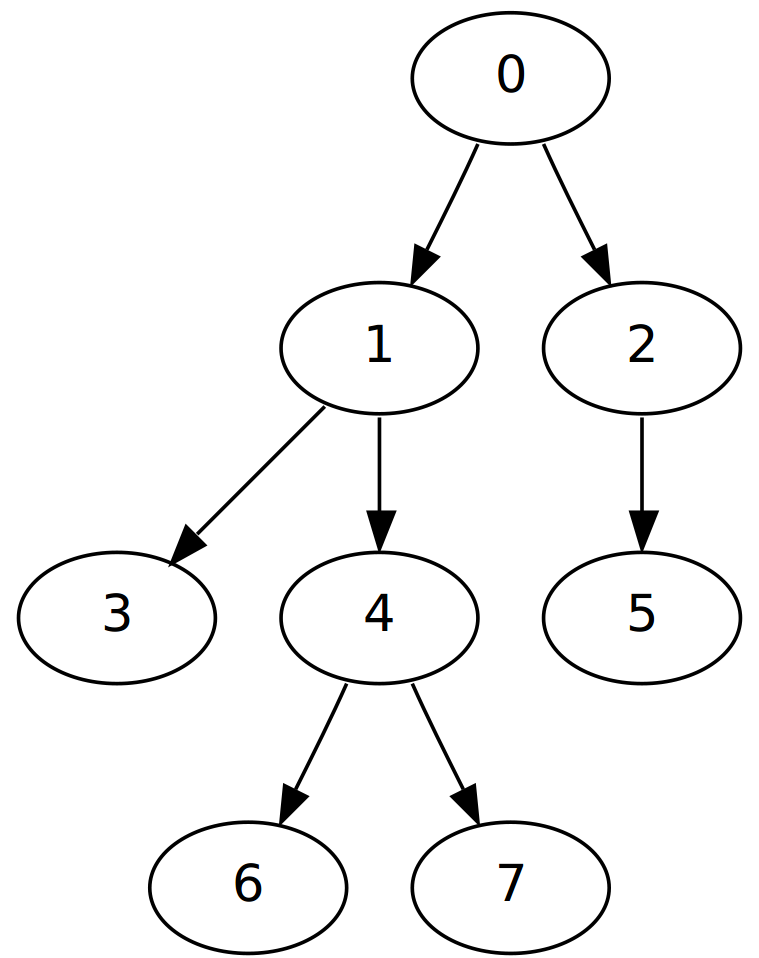
\includegraphics[height=4cm, width=3cm]{srj-figures/tracelet.png}
	\caption{Control-flow graph (CFG) of a sample fucntion}\label{fig:tracelet}
\end{figure}

\begin{table}[!ht]
\caption{Partial traces generated from a sample fucntion CFG shown in figure \ref{fig:tracelet}}\label{tab:par_tra}
\begin{center}
{\scriptsize
\begin{tabular}{|c|c|}
  \hline
  \textbf{$k$} & \textbf{Generated partial traces} \\
  \hline
  1 & $\langle 0 \rangle$, $\langle 1 \rangle$, $\langle 2 \rangle$, $\langle 3 \rangle$, $\langle4\rangle$, $\langle 5 \rangle$, $\langle 6 \rangle$, $\langle 7 \rangle$\\
  \hline
  2 & $\langle 0,1 \rangle$, $\langle 1,3 \rangle$, $\langle 1,4 \rangle$, $\langle 4,6 \rangle$, $\langle 4,7 \rangle$, $\langle 0,2 \rangle$, $\langle 2,5 \rangle$\\
  \hline
  3 & $\langle 0,1,3 \rangle$, $\langle 0,1,4 \rangle$, $\langle 1,4,6 \rangle$, $\langle 1,4,7 \rangle$, $\langle 0,2,5 \rangle$\\
  \hline
  \end{tabular}
}
\end{center}
\end{table}

\begin{table}[!ht]
\caption{Function models constructed from partial traces shown in Table \ref{tab:par_tra}}\label{tab:func_mod}
\begin{center}
{\scriptsize
\begin{tabular}{|m{0.2cm}|m{5.5cm}|m{0.5cm}|}%{|c|c|}
  \hline
  \textbf{$n$} & \textbf{Constructed function models} & \textbf{$w_n$}\\
  \hline
  1 & $\langle 0 \rangle$, $\langle 1 \rangle$, $\langle 2 \rangle$, $\langle 3 \rangle$, $\langle4\rangle$, $\langle 5 \rangle$, $\langle 6 \rangle$, $\langle 7 \rangle$ & 0.500\\
  \hline
  2 & $\langle 0,1 \rangle$, $\langle 1,3 \rangle$, $\langle 1,4 \rangle$, $\langle 4,6 \rangle$, $\langle 4,7 \rangle$, $\langle 0,2 \rangle$, $\langle 2,5 \rangle$ & 0.750\\
  \hline
  3 & $\langle 0,1,3 \rangle$, $\langle 0,1,4 \rangle$, $\langle 1,4,6 \rangle$, $\langle 1,4,7 \rangle$, $\langle 0,2,5 \rangle$ & 0.830\\
  \hline
    4 & $\langle 0 \rangle$, $\langle 1 \rangle$, $\langle 2 \rangle$, $\langle 3 \rangle$, $\langle4\rangle$, $\langle 5 \rangle$, $\langle 6 \rangle$, $\langle 7 \rangle$, $\langle 0,1 \rangle$, $\langle 1,3 \rangle$, $\langle 1,4 \rangle$, $\langle 4,6 \rangle$, $\langle 4,7 \rangle$, $\langle 0,2 \rangle$, $\langle 2,5 \rangle$ & 0.625\\
  \hline
  5 & $\langle 0,1 \rangle$, $\langle 1,3 \rangle$, $\langle 1,4 \rangle$, $\langle 4,6 \rangle$, $\langle 4,7 \rangle$, $\langle 0,2 \rangle$, $\langle 2,5 \rangle$, $\langle 0,1,3 \rangle$, $\langle 0,1,4 \rangle$, $\langle 1,4,6 \rangle$, $\langle 1,4,7 \rangle$, $\langle 0,2,5 \rangle$ & 0.790\\
  \hline
  6 & $\langle 0,1,3 \rangle$, $\langle 0,1,4 \rangle$, $\langle 1,4,6 \rangle$, $\langle 1,4,7 \rangle$, $\langle 0,2,5 \rangle$, $\langle 0 \rangle$, $\langle 1 \rangle$, $\langle 2 \rangle$, $\langle 3 \rangle$, $\langle4\rangle$, $\langle 5 \rangle$, $\langle 6 \rangle$, $\langle 7 \rangle$ & 0.665\\
  \hline
  7 & $\langle 0,1 \rangle$, $\langle 1,3 \rangle$, $\langle 1,4 \rangle$, $\langle 4,6 \rangle$, $\langle 4,7 \rangle$, $\langle 0,2 \rangle$, $\langle 2,5 \rangle$, $\langle 0 \rangle$, $\langle 1 \rangle$, $\langle 2 \rangle$, $\langle 3 \rangle$, $\langle4\rangle$, $\langle 5 \rangle$, $\langle 6 \rangle$, $\langle 7 \rangle$, $\langle 0,1,3 \rangle$, $\langle 0,1,4 \rangle$, $\langle 1,4,6 \rangle$, $\langle 1,4,7 \rangle$, $\langle 0,2,5 \rangle$ & 0.693\\
  \hline

  \end{tabular}
}
\end{center}
\end{table}

Unfortunately, compiler optimizations and/or difference in build environments often lead to changes in the basic-block structure. Thus, basic-block based function modelling is not preferred\footnote{Basic-block based modelling refers to single basic-block based function models.}.  For example, given a search query that consists of a single basic block, we may miss similar functions in the target function pool due to structural difference, where target functions can be of several basic-blocks and the similarity between the query function and each of the basic-blocks in the target functions can be below the pre-defined threshold value. This is a common observation that arises due to compiler optimization techniques that lead to basic-block splitting (or merging) and function inclining (or outlining). Hence, in \tool, we use partial traces of various lengths to model the functions. 

The key advantage of partial trace modelling, over other techniques, is that it is resilient to the structural changes incurred by the aforementioned compiler optimization techniques, which might negatively influence the similarity search. That is, partial traces generated at various lengths from the search query function are matched against the partial traces of different lengths generated from the functions in the target function pool. However, in generating partial traces, one must ensure that the generated partial traces are valid or feasible during real-world executions. To this end, we propose a \textit{pruning} technique to remove partial traces that are \textit{infeasible} in practise. %\note{absolutely}

\subsubsection{Pruning of Partial Traces} \label{subsubsec:sou_prun}

%\note{THEOREM 2. Given a template T , an oracle, and any nsyn ,
%nver , if T is sufficient for abstracting φ, then the procedure
%DInputVal(, T, nsyn , nver ) returns a function C semantically
%equivalent to .
%A useful corollary is that, if the procedure DInputVal returns “In-
%sufficient Template” for any nsyn , nver , then the template T is in-
%deed insufficient for abstracting φ. However, this theorem is weaker
%than Theorem 1 as it does not guarantee that the procedure returns
%“Insufficient Template” whenever the template is insufficient.
%Just like procedure ExhaustVal, DInputVal provides a satis- \\
%}


\tool is a static analysis based tool and hence, it is relatively difficult (or impossible) to identify all the partial traces that are infeasible in practise. In \tool, we prune partial traces that are infeasible with the help of the theorem prover. That is, given a partial trace, we extract symbolic expressions, as explained in Section~\ref{subsec:fea_ext}, and pass them to the solver, which will try to solve the constraints and generate a model that satisfies them all. If the solver fails to generate a model, we label that partial trace as infeasible and prune it from the analysis. It is also noted that the partial traces, for which the solver is able to generate a model, may too become infeasible during real world execution as the feasibility of a path depends on various factors, such as global variables, values in the heap and other dynamic data, that are beyond the scope of static analysis.
Infeasible path elimination is a difficult task even in dynamic analysis. Comparing to the static analysis solutions proposed in the literature \cite{david2014tracelet,pewny2014leveraging,pewnycross}, this work makes an attempt to reduce the searching candidates using SMT solvers.

%\note{On the other hand, if a solver is unable to generate a model for a partial trace then it is indeed infeasible as there are no real values that can be substituted for the symbolic variables (i.e., symbolic registers, flags and memory locations) such that all the constraints are solved. Even though we are unable to prune all the infeasible partial traces, comparing to the static analysis solutions proposed in the literature \cite{david2014tracelet,pewny2014leveraging,pewnycross}, we are heading towards the right direction of eliminating infeasible paths in analysis.}

Even with the infeasible partial traces pruned, it is still difficult to compare search query function against each functions  in the target function pool as there must be a systematic way to do the comparison. That is, the question ``what lengths of partial traces in the search query need to be compared against what lengths of partial traces in the target function pool?'' still persists. To this end, we propose a simple function modelling technique to represent each function using partial traces of various lengths.

\subsubsection{Function Modelling} \label{subsubsec:fun_mod}

It is understood that partial traces need to be organized in a systematic way to effectively compare two different functions. In \tool, for each function, we construct function models by combining partial traces of different lengths.
\begin{mydef}
\emph{\textbf{(Function model)}} It is a unique combination of partial traces, of various lengths, constructed for each function. Given the lengths of partial traces are $\mathtt{k}$, in total, $\mathtt{2^k-1}$ function models are constructed from each function.
\end{mydef}

For example, partial traces of three different lengths (i.e., $k=1,2,3$), generated from the function CFG shown in Fig.~\ref{fig:tracelet}) is presented in Table~\ref{tab:par_tra}. From the table, it can be seen that there are, in total, 20 partial traces are generated from the function. 
From the partial traces presented in Table~\ref{tab:par_tra} (assuming all the partial traces are feasible), 7 (i.e., $N=2^3-1$) function models are constructed and they are listed in Table~\ref{tab:func_mod}. For example, from the table, it can be seen that function model 1 consists of partial traces of length 1, model 4 consists of partial traces of lengths 1 and 2, and model 7 consists of all partial traces.

One might argue that function model 7 alone would be sufficient as it contains all the partial traces. However, it is observed that having more than required partial traces may lead to higher false positive rate. This is due to the fact that, in \tool, as explained in section \ref{subsubsec:sb_sem_mod_fe}, a constraint solver is used to solve the symbolic expressions. Given the complexity of constraints there can be more than one possible assignments to symbolic arguments that can satisfy all the constraints. That is, given the constraints are too trivial to solve, input arguments present in two different symbolic expressions might be assigned the same values, which, in this case, considered false positive.

For example, consider the following two `toy' constraints obtain from two different partial traces:
\begin{eqnarray}
\mathtt{0x10 = eax+ebx} \label{eq:cons_1} \\
\mathtt{0x10 = ecx-edx} \label{eq:cons_2}
\end{eqnarray}
From the Equations \ref{eq:cons_1} and \ref{eq:cons_2}, we can see that they are quite trivial and the symbolic registers $\mathtt{\langle eax,ebx\rangle}$ and $\mathtt{\langle ecx,edx\rangle}$ can possibly have too many satisfying assignments. Interestingly, the default satisfying model generated by Z3 solver for Equation \ref{eq:cons_1} is $\mathtt{eax=0x10}$ and $\mathtt{ebx=0x00}$, and for Equation \ref{eq:cons_2} is $\mathtt{ecx=0x10}$ and $\mathtt{edx=0x00}$. Therefore, given the values assigned to the symbolic registers, both the partial traces have the same effect on the program state and hence, considered similar, which is false. It is noted that, in \tool, we abstract away the register name to account for various register names used across multiple architectures. Thus, the assignments $\mathtt{eax=0x10}$ and $\mathtt{ecx=0x10}$ are considered same, where the value $\mathtt{0x10}$ is assigned to a register.

To address the aforementioned issue, in function model matching (discussed in Section~\ref{subsec:fun_mod_mat}), we encourage matching between function models that are composed of larger partial traces by assigning different weights to each model. That is, function model matching between larger partial traces has higher weights than the smaller partial traces. This is based on the observation that larger partial traces tend to have complex constraints, which limits the number of possible satisfying assignment to symbolic variables and hence, reduce the false positive rate. The weights for function models are assigned using Equation~\ref{eq:wei_ass}.
\begin{eqnarray}
\mathtt{w_n=\frac{1}{\vert K_n \vert}\sum_{\substack{\mathtt{k} \in \mathtt{K_n}}}\left(1-\frac{1}{2*k} \right)} \label{eq:wei_ass}
\end{eqnarray}
Here, $\mathtt{w_n}$ refers to the weight assigned to function model $n$ and $\mathtt{K_n}$ refers to the set of different partial trace types (in terms of length) present in function model $n$. For example, the weight for function model 7 ($\mathtt{w_7}$) is determined as follows: there are three types of partial traces (i.e., $\mathtt{K_7={1,2,3}}$) and the individual weights for partial trace lengths 1, 2 and 3 are $\mathtt{0.50, 0,75}$ and $\mathtt{0.83}$, respectively, finally, the combined weight is calculated to be $\mathtt{0.693}$ ($=\mathtt{(0.50+0.75+0.83)/3}$).

\subsection{Function Model Matching} \label{subsec:fun_mod_mat}

One of the key advantages of function model is that it enables \textit{n-to-m}, \textit{1-to-n}, \textit{n-to-1} and \textit{1-to-1} matches across the signature\footnote{Here signature function refers to the search query function in hand} and target functions\footnote{Similarly, target functions refer to functions in the target binary pool against which the signature function is matched}, eliminating the effects of compiler optimizations and differences in compilers.

\begin{description}
  \item[\textit{n-to-m}] Partial traces of the length $n (\in\mathbb Z_{> 1})$ generated from the signature function are matched against the partial traces of the length $m (\in\mathbb Z_{> 1})$ generated from target function.
  \item[\textit{1-to-n}] Each basic-block (i.e., partial trace of the length 1) in the signature function is matched against the partial traces of the $n (\in\mathbb Z_{> 1})$ generated from target function.
  \item[\textit{n-to-1}] Partial traces of the length $n (\in\mathbb Z_{> 1})$ generated from the signature function are matched against each basic-block in the target function.
  \item[\textit{1-to-1}] Each basic-block in the signature function is matched against each basic-block in the target function. It is also known as pairwise comparison of basic-blocks.
\end{description}

Among the four types of matching, \textit{1-to-n} matching addresses the issue of basic-block splitting, that is, a single basic-block in the signature function is split into several smaller basic-blocks in the target function. Similarly, \textit{n-to-1} matching addresses the basic-block merging problem. On the other hand, \textit{n-to-m} mapping is generally preferred when the signature (target) function is part of a huge target (signature) function and appropriately selected values for $n$ and $m$ will maximize the function similarity. Finally, if non of the aforementioned matching techniques work, \textit{1-to-1} matching is performed to compare the pairwise basic-block similarity.

It is noted that in \tool, the function model matching is not fixed, where, for a given signature function, the searching algorithm will try all possible function models and pick the best one that maximizes the signature-target function similarity. In contrast, the techniques proposed in the literature do not have the flexibility to try out all possible matchings. For example, in tracelet-based modelling \cite{david2014tracelet}, the authors recommended that the tracelet size should be larger (e.g., $k>2$), for both signature and target functions, hence, only \textit{n-to-m} matching is performed, in fact, it is \textit{n-to-n} matching as they consider same tracelet size for both signature and target functions. Further, in \cite{pewnycross} and \cite{luo2014semantics}, pairwise comparison of basic-blocks (i.e., \textit{1-to-1} matching) is performed as an initial step to identify potential target functions, which inherently assumes that the program structure is maintained across signature and target functions and at least one basic-block in the target function resembles a basic-block in the signature function.

%\subsubsection{Similarity measure} \label{subsubsec:sim_mea}
%During function model matching process, the similarity between different function models (e.g., $f_a$ and $f_b$) is measured using Jaccard distance:
%\begin{equation}
%\begin{aligned}
%Jaccard(f_a, f_b) = \frac{\vert f_a \cap f_b \vert}{\vert f_a \cup f_b \vert}
%\end{aligned}
%\end{equation}

\subsubsection{Example} \label{subsubsec:exp}

\begin{figure}
\centering
\noindent
\begin{minipage}{.11\textwidth}
\begin{lstlisting}[caption=BB1,frame=tlrb]{Name}
push ebp
mov ebp, esp
\end{lstlisting}
\end{minipage}\hfill
\begin{minipage}{.11\textwidth}
\begin{lstlisting}[caption=BB2,frame=tlrb]{Name}
pop ebx
mov ecx, ebx
\end{lstlisting}
\end{minipage}\hfill
\begin{minipage}{.15\textwidth}
\begin{lstlisting}[caption=sym. expr for BB1 (partial trace with length 1),frame=tlrb]{Name}
ESP' = ESP - 0x4
[ESP - 0x4] = EBP
EBP = ESP - 0x4
\end{lstlisting}
\end{minipage}\hfill

\begin{minipage}{.15\textwidth}
\begin{lstlisting}[caption=sym. expr for BB2 (partial trace with length 1),frame=tlrb]{Name}
ESP' = ESP + 0x4
EBX = [ESP]
ECX = [ESP]
\end{lstlisting}
\end{minipage}\hfill
\begin{minipage}{.20\textwidth}
\begin{lstlisting}[caption=sym. expr for both BBs combined (partial trace with length 2),frame=tlrb]{Name}
ESP' = ESP - 0x4 + 0x4
[ESP - 0x4] = EBP
EBP = ESP - 0x4
EBX = [ESP - 0x4]
ECX = [ESP - 0x4]
\end{lstlisting}
\end{minipage}
\caption{Sample basic-blocks and their corresponding symbolic expressions at two different granularity levels} \label{fig:sym_expr_granu}
\end{figure}

Figure \ref{fig:sym_expr_granu} depicts the sample basic-blocks (assuming they are adjacent and lie along the execution path in a function CFG) and the corresponding symbolic expressions extracted for partial traces of the length $1$ and $2$, denoted as PT-1 and PT-2, respectively. From the example, it can be seen that \texttt{ESP}, \texttt{EBX} and \texttt{ECX} registers hold different values in PT-2 model (see listing 5) compare to PT-1 model (see listing 3 and 4). That is, when two basic-blocks are merged, the extracted semantic features change considerably, which in return, will have an adversarial effect in vulnerability signature matching process. Thus, it is vital to extract semantic features at a suitable granularity level such that the vulnerabilities are not missed.

\subsection{Locality Sensitive Hashing} \label{subsec:lsh}
In \tool, we leverage on Locality-sensitive Hashing (LSH) technique to perform the function matching more efficiently and in a scalable manner. Locality-sensitive hashing is an algorithm for searching similar items in large and high dimensional dataset \cite{DBLP:books/cu/LeskovecRU14} based on the assumption that, if two items are similar, the hashed value of the two items will remain similar. In \tool, we use MinHashing \cite{Broder:1997:RCD:829502.830043} technique to hash the extracted features and generate hash signature for each function model. To this end, we use 1000 (i.e., $n=1000$) hash functions to generate the signature, which leads to an error of 3.16\%. The similarity between two function model is given by this equation: 
\begin{equation}
\begin{aligned}
 sim(mh_a, mh_b) = \frac{\vert mh_a[i]=mh_b[i ]\vert}{n}
\end{aligned}
\end{equation}

where the jaccard similarity between two function models is approximated by the MinHash similarity between the functions models


\subsection{Post-processing} \label{subsubsec:post-proc}
One challenge in matching smaller functions is that the number of semantic features that can be extracted is very limited, which may lead to a high false positive rate. This is one of the key limitations for static analysis based on function modelling techniques~\cite{david2014tracelet,pewnycross}. For example, in \cite{david2014tracelet}, all the functions need to satisfy the minimum basic-blocks requirement, where functions with less than 100 basic-blocks are ignored from the analysis. We find this requirement is very restrictive in real-world applications. For example, in \texttt{msvcrt.dll}, the \texttt{strlen} function has only 14 basic-blocks, and also the same function has only 20 basic-blocks in \texttt{libc}.

Hence, in \tool, we add a post-processing step that removes the limitation of matching (or searching) small functions. In post-processing process, we clear up the search results by removing the false positives. To this end, we leverage on clustering technique to identify false positives. That is, from the initial search results (i.e., before post-processing), we extract all the function names that appear within top 500 ranks\footnote{If the search results contain less than 500 functions, we take the entire results.}. Extracting function names at the binary level is possible as our target function pool contains only open-source binaries and in general, function name indicates the high-level functionality of a functions \note{cite ref}. Later, from the extracted function names, treating them as some random strings, we construct n-grams models of various lengths. In \tool, we construct tri-gram ($n=3$) and four-gram ($n=4$) models from each function name and use them as features to do the clustering. For example, features extracted from the function name \texttt{strlen} is as follows:
\begin{eqnarray}
\mathtt{F_3 = \lbrace str,trl,rle,len\rbrace}  \\
\mathtt{F_4 = \lbrace strl,trle,rlen\rbrace}
\end{eqnarray}

Here, $\mathtt{F_3}$ and $\mathtt{F_4}$ refer to tri-gram and four-gram features, respectively. Once the clustering is done, we remove the clusters with only 1 element (or function name), where a cluster with 1 (or very few) elements is considered `outlier' in machine learning terminology. It is important to note that, using this technique, we can only remove completely unrelated functions (or outliers) from the search results and cannot remove the functions that appear similar to the search query at the function name-level (e.g., \texttt{strlen} vs. \texttt{strcpy}). Even though, post-processing module can only remove outliers, we find this very useful as it completely removes the unwanted results and keep only the related ones (at least at the function name-level). We remark that it is possible incorporate more domain specific heuristics in this module to further improve the accuracy, e.g., .
